Historically, dxex is based on PythonPDEVS~\cite{PythonPDEVS}.
Python is a good language for prototypes, but performance has proven insufficient to compete with other simulation kernels~\cite{MasterThesis}.
Dxex is a C++11-based implementation of PythonPDEVS, but implements only a subset of PythonPDEVS, whiel making some of its own additions.
So while the feature set is not too comparable, the architectural design, core simulation algorithm, and optimizations, are highly similar.

We will not make a detailed comparison with PythonPDEVS here, but only mention some supported features.
Dxex supports, similarly to PythonPDEVS, the following features: direct connection~\cite{SymbolicFlattening}, \textsf{Dynamic Structure DEVS}~\cite{DSDEVS}, termination conditions, and a modular tracing and scheduling framework~\cite{PythonPDEVS}.
But whereas PythonPDEVS only supports optimistic synchronization, dxex support multiple synchronization protocols (though only in parallel).
This is in line with the design principle of PythonPDEVS: allow users to pass performance hints to the simulation kernel.
In our case, a user can pass the simulation kernel the ``hint'' as to which synchronization protocol must be used for this model.
Our implementation in C++11 also allows for optimizations which were plainly impossible in an interpreted language.

Since there is no universal \textsf{DEVS} model standard, dxex models are incompatible with PythonPDEVS and vice versa.
This is due to dxex models being grafted on C++11, whereas PythonPDEVS models are grafted on Python.

In the remainder of this section, we will elaborate on our prominent new feature: support for multiple synchronization protocols within the same simulation tool, which are offered transparantly to the model.

\subsection{Synchronization protocols}
We previously explained the existence of different synchronization protocols exist, each optimized for a specific kind of model.
As no single synchronization protocol is ideal for all models, a general purpose simulation tool should support multiple protocols.
Currently, most parallel simulation tools chose only a single synchronization protocol due to the inherent differences between protocols.
An uninformed choice on which one to implement is insufficient, as performance will likely be bad.
We argue that a real general purpose simulation tool should support sequential, conservative, and optimistic synchronization, as is the case for dxex.

These different protocols relate to three different model characteristics.
Conservative synchronization for when high lookahead exists between different nodes, and barely any blocking is necessary.
Optimistic synchronization for when lookahead is unpredictable, or there are rare (almost) instantaneous events.
Finally, sequential simulation is still required for models where parallelism is bad, where all protocols actually slow down simulation.

\subsubsection{Sequential}
Our sequential simulation algorithm is very similar to the one found in PythonPDEVS, including many optimizations.
Minor modifications were made, though, such that it can be overloaded by different synchronization protocol implementations.
This way, the \textsf{DEVS} simulation algorithm is implemented once, but parts can be overridden as needed.
In theory, more synchronization protocols (\textit{e.g.}, other algorithms for conservative synchronization) can be added without altering our design.

An overview of dxex's design is given in Figure~\ref{fig:class_diagram}.
It shows that there is a simulation \texttt{Core}, which simulates the \texttt{AtomicModel}s connected to it.
The superclass \texttt{Core} is merely the sequential simulation core, but can be used as-is.
Subclasses define specific variants, such as \texttt{ConservativeCore} (conservative synchronization), \texttt{OptimisticCore} (optimistic synchronization), and \texttt{DynamicCore} (\textsf{Dynamic Structure DEVS}).

\begin{figure}
    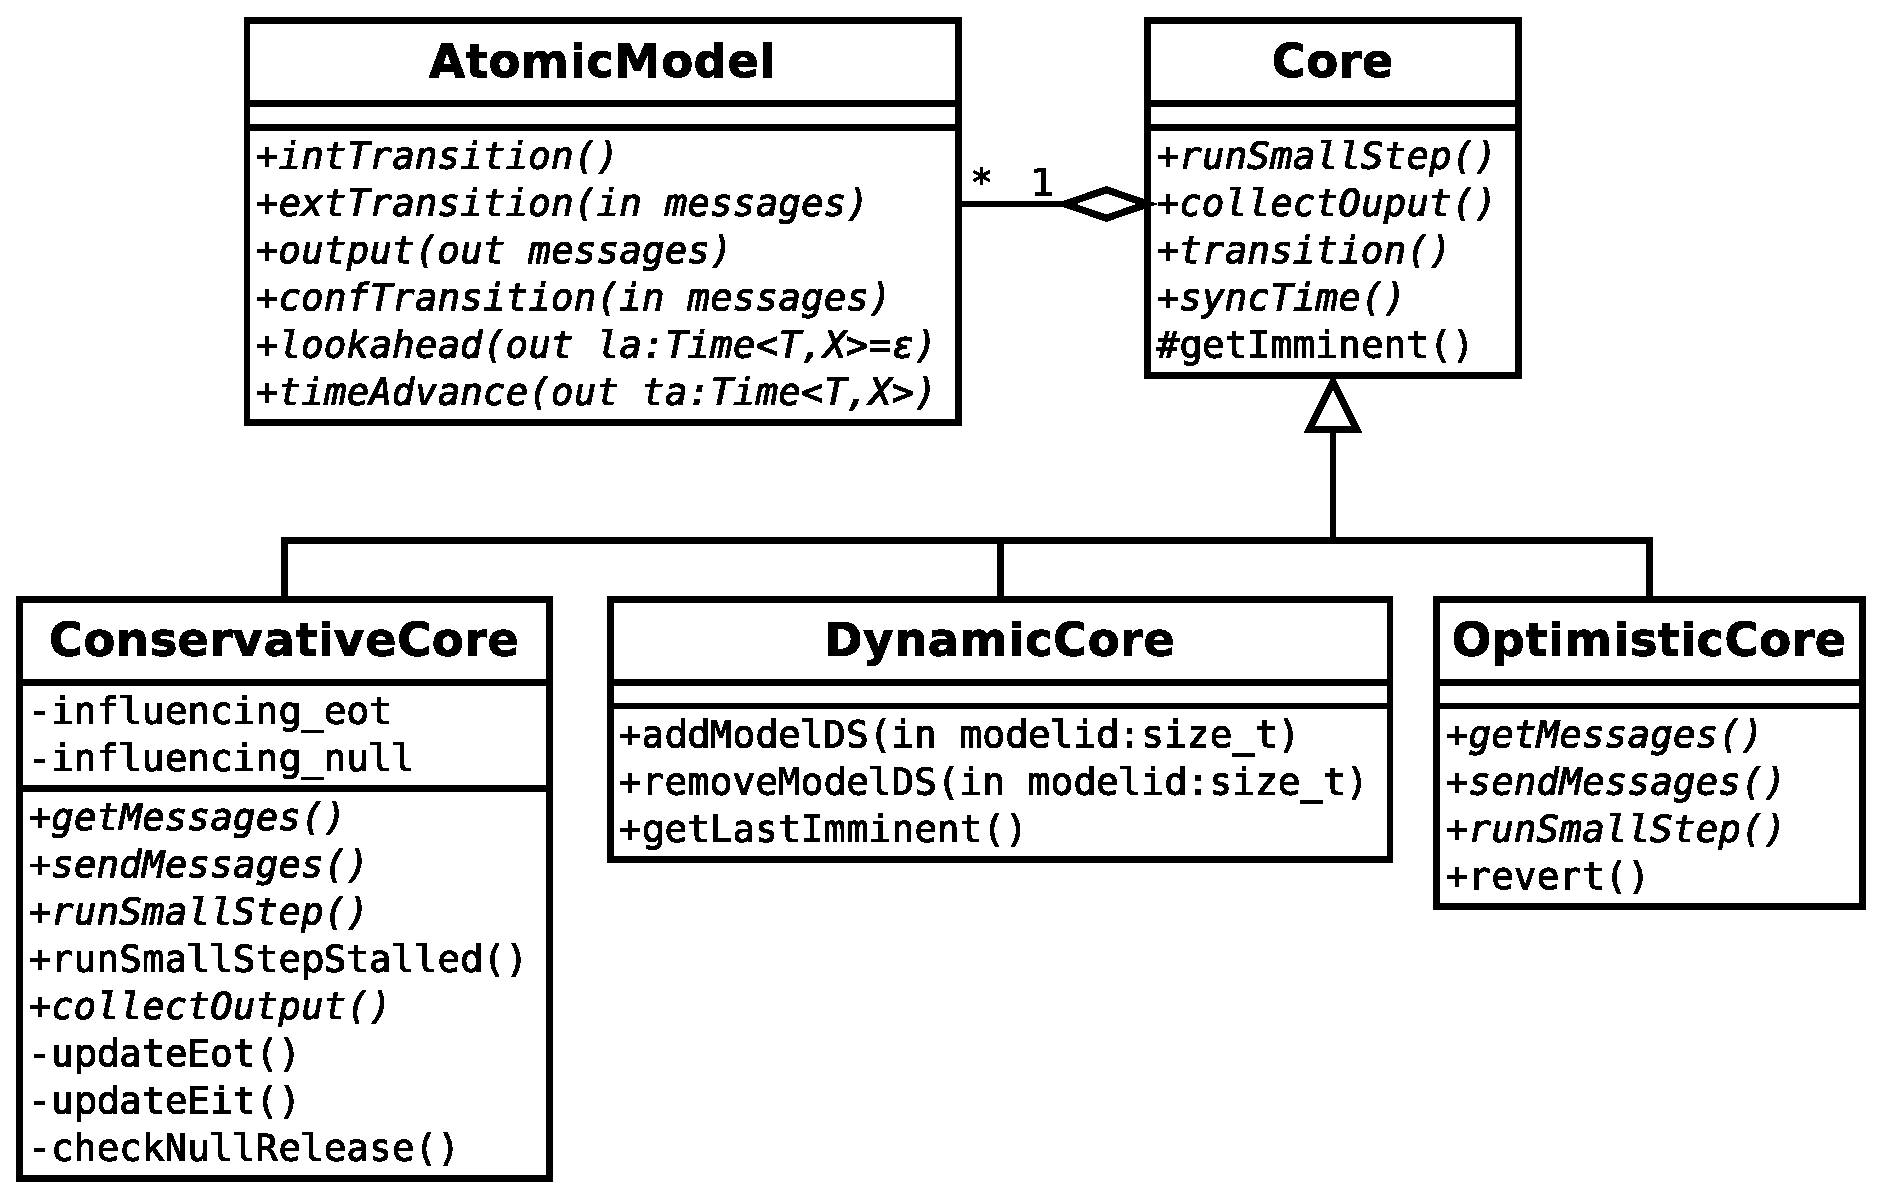
\includegraphics[width=\columnwidth]{fig/cores_class_diagram.eps}
	\caption{Dxex kernel design.}
	\label{fig:class_diagram}
\end{figure}

\subsubsection{Conservative}
For conservative synchronization, each node must determine the nodes it is influenced by.
Each model needs to provide a lookahead function, which determines the lookahead depending on the current simulation state.
Within the returned time interval, the model promises not to raise an event.
A node aggregates this information to computes its earliest output time (EOT).
This value is written out in shared memory, where it can be read out by all other nodes.

Reading and writing to shared memory is done through the use of the new C++11 synchronization primitives.
Whereas this was also possible in previous versions of the C++ standard, by falling back to non-portable C functions, it was not a part of the C++ language standard.
C++11 further allows us to make the implementation portable, as well as more efficient: the compiler might know of optimizations specific to atomic variables.

\subsubsection{Optimistic}
For optimistic synchronization, each node must be able to roll back to a previous point in time.
This is often implemented through the use of state saving.
This needs to be done carefully in order to avoid unnecessary copies, and minimize the overhead.
We use the default: explicitly save each and every intermediate state.
Mattern's algorithm~\cite{mattern} is used to determine the GVT, as it runs asynchronously and uses only $2n$ synchronization messages.
Once the GVT is found, all nodes are informed of the new value, after which fossil collection is performed, and irreversible actions are committed.

The main problem we encountered in our implementation is the aggressive use of memory.
Frequent memory allocation and deallocation caused significant overheads, certainly when multiple threads do so concurrently.
This made us switch to the use of thread-local (using \texttt{tcmalloc}) memory pools.
Again, we made use of specific new features of C++11, that were not available in Python, or even previous versions of the C++ language standard.

\subsection{Transparency}
We define simulation kernel transparancy as having a single model, which always can be executed on each supported synchronization kernel, without any modifications.
User should thus only provide one model, implemented in C++11, which can be either using sequential execution, using conservative synchronization, or using optimistic synchronization.
Switching between simulation kernels is as simple as altering the simulation termination time.
The exception is conservative synchronization, where a lookahead function is required, which is not used in other synchronization kernels.
Two options are possible: either a lookahead function must always be provided, even when it is not required and possibly not used, or we use a default lookahead function if none is defined.

Always defining a lookahead function might seem redundant, especially if users will never use conservative synchronization.
Especially since defining the lookahead is often non-trivial and dependent on intricate model details.
The more attractive option is for the simulation tool to provide a default lookahead function, such that simulation can run anyway, but maybe not at peak performance.
Depending on the model, simulation performance might still be faster than sequential simulation.

Defining a lookahead function is therefore recommended in combination with conservative synchronization, but is not a necessity, as a default can be used otherwise.
